\documentclass[11pt, a4paper, twoside, a4wide, headsepline, bibtotoc]{report}
\textwidth = 16cm
\textheight = 23,7cm
\topmargin = 0pt
\marginparsep = 0pt
\marginparwidth = 0pt
\footskip = 1cm
\voffset = 0pt
\headsep = 0cm
\oddsidemargin 1cm
\evensidemargin 0cm

\usepackage[portuges]{babel}

\usepackage{enumitem}
\setlist{nolistsep}
\setlist{noitemsep}

\usepackage{sectsty}
% Para letras sans serif para os títulos das secções
\allsectionsfont{\usefont{OT1}{phv}{bc}{n}\selectfont}

\usepackage{color}
\definecolor{dkgreen}{rgb}{0,0.6,0}
\definecolor{gray}{rgb}{0.5,0.5,0.5}
\definecolor{mauve}{rgb}{0.58,0,0.82}
\definecolor{rltbrightred}{rgb}{1,0,0}
\definecolor{rltred}{rgb}{0.75,0,0}
\definecolor{rltdarkred}{rgb}{0.5,0,0}
\definecolor{rltbrightgreen}{rgb}{0,0.75,0}
\definecolor{rltgreen}{rgb}{0,0.5,0}
\definecolor{rltdarkgreen}{rgb}{0,0,0.25}
\definecolor{rltbrightblue}{rgb}{0,0,1}
\definecolor{rltblue}{rgb}{0,0,0.75}
\definecolor{rltdarkblue}{rgb}{0,0,0.5}
\definecolor{webred}{rgb}{0.5,.25,0}
\definecolor{webblue}{rgb}{0,0,0.75}
\definecolor{webgreen}{rgb}{0,0.5,0}
\definecolor{webbrightgreen}{rgb}{0,0.5,0}


\usepackage[pdftex,
colorlinks=true,
urlcolor=rltblue,               % \href{...}{...}
anchorcolor=rltbrightblue,
filecolor=rltgreen,             % \href*{...}
linkcolor=rltblue,               % \ref{...} and \pageref{...}
menucolor=webdarkblue,
citecolor=webbrightgreen,
pdftitle={Relatorio},
pdfauthor={Pedro Moreira},
pdfsubject={Programação Centrada na Rede},
pdfkeywords={UML, Diagrama de Classes, Diagrama de Sequencia, Interface, PHP, usabilidade, acessibilidade, html, smarty, mySQL},
pagebackref=false,
pdfpagemode=None,
bookmarksopen=true]{hyperref}
\pdfcompresslevel=9
\linespread{1.3} % espaçamento de linha e meia


\bibliographystyle{plain}
\usepackage[pdftex]{graphicx}
 \usepackage{thumbpdf}

\newcommand{\goodgap}{%
\hspace{\subfigtopskip}%
\hspace{\subfigbottomskip}}
% processamento mais agradável de figuras
\renewcommand{\topfraction}{0.85}
\renewcommand{\textfraction}{0.1}
\renewcommand{\floatpagefraction}{0.75}

\usepackage{icomma}
\usepackage[utf8x]{inputenc} 

\usepackage{makeidx}
\usepackage{listings}
\usepackage[isu,small,ruled]{caption}
%\setlength{\captionmargin}{0.5cm}
\usepackage{prettyref}

\newcommand\glossaryname{Gloss{\'a}rio}
\newrefformat{fig}{Figura~\ref{#1}}

\definecolor{dkgreen}{rgb}{0,0.6,0}
\definecolor{gray}{rgb}{0.5,0.5,0.5}
\definecolor{mauve}{rgb}{0.58,0,0.82}


\newcommand{\HRule}{\rule{\linewidth}{0.5mm}}



\title{Programação Centrada na Rede}
\author{Pedro Moreira}
\usepackage{datetime}
\newdate{date}{23}{09}{2013}
\date{\displaydate{date}}

%\usepackage{listings}
\usepackage{color}

\definecolor{dkgreen}{rgb}{0,0.6,0}
\definecolor{gray}{rgb}{0.5,0.5,0.5}
\definecolor{mauve}{rgb}{0.58,0,0.82}

\lstset{frame=tb,
  language=PHP,
  aboveskip=3mm,
  belowskip=3mm,
  showstringspaces=false,
  columns=flexible,
  basicstyle={\small\ttfamily},
  numbers=none,
  numberstyle=\tiny\color{gray},
  keywordstyle=\color{blue},
  commentstyle=\color{dkgreen},
  stringstyle=\color{mauve},
  breaklines=true,
  breakatwhitespace=true,
  tabsize=2
}

\begin{document}
%\renewcommand{\chaptername}{}
%\renewcommand{\thechapter}{}
%\renewcommand{\thesection}{}
%\renewcommand{\thesubsection}{}
%\renewcommand{\thesubsubsection}{}
%\setcounter{secnumdepth}{-1}

\newcommand{\code}[1]{\lstinline{#1}}
%\lstset{
 % breaklines=no
%}


%\input{ante_rosto}
\setcounter{page}{1}
\pagenumbering{arabic}
\begin{titlepage}

\begin{center}

% Upper part of the page

\includegraphics[width=0.15\textwidth]{logo.png}\\[1cm]    


\textsc{\LARGE Instituto Politécnico de Beja\\Escola Superior de Tecnologia e Gestão}\\[1.5cm]
\textsc{Licenciatura em Engenharia Informática}\\
\textsc{Programação Centrada na Rede}




% Title
\topskip0pt
\vspace*{\fill}
\textsc{Projecto da Disciplina - Fases de Desenho e Implementação}\\*
{\huge \bfseries SISTEMA DE GESTÃO\\*
 \bfseries DE MOMENTOS DE AVALIAÇÃO}\\*[0cm]
\textsc{Ano lectivo: 2012/2013 / 2º Semestre / 3º ano}
\vspace*{\fill}


\vfill

% Bottom of the page
{
% Author and supervisor
\emph{Aluno:} Pedro \textsc{Moreira} N.10015\\



\emph{Docente:} Luís \textsc{Bruno}
\\

\large \today

}

\end{center}
\end{titlepage}
%\maketitle						% automatic title!

\cleardoublepage
\addcontentsline{toc}{chapter}{Índice Geral}
\tableofcontents
\addcontentsline{toc}{chapter}{Lista de Figuras}
\listoffigures
\cleardoublepage



\chapter{Introdução}

\paragraph{}

\section{Objectivos}
Este relatório insere-se na avaliação da disciplina "Programação Centrada na Rede", leccionada no 2º semestre do 3º ano da licenciatura em Engenharia Informática.\\ 
O trabalho surge na sequência do projecto interdicsiplinar de Engenharia de Software, Bases de Dados I e II, Hipermédia e Acessibilidade e, por último, Programação Centrada na Rede.\\
O tema é o desenvolvimento de uma aplicação que permita gerir os momentos de avaliação das diferentes disciplinas dos cursos da Estig.
Nele pretende-se apresentar um resumo da análise e a fase de desenho do desenvolvimento da aplicação.\\

\section{Problema}
Actualmente, cada docente marca as suas diferentes avaliações de forma individual, podendo ou não enviar essa informação ao Coordenador de Curso. Este, para ter noção da distribuição de carga dos momentos de avaliação ao longo de um semestre tem que, manualmente, registar essa informação, que poderá ser alterada posteriomente, sem que ele receba qualquer notificação. Por outro lado não existe um repositório que centralize todos os momentos de avaliação realizados nas disciplinas ao longo do semestre e que seja transparente para os seus diferentes beneficiários.

\section{Objectivos}
Neste projecto pretende-se a criação de uma aplicação que centralize o registo de todos os momentos de avaliação mantendo os respectivos intervenientes actualizados acerca das alterações às mesmas.\\
Por forma a evitar uma carga excessiva aos alunos, as avaliações terão obrigatóriariamente que ser analisadas pelo coordenador do curso em causa.\\
Na aplicação será também implementada forma para facilitar a percepção do estado das avaliações por parte dos actores.\\





\chapter{Descrição Geral}

\paragraph{}

\section{Perspectiva}
Este trabalho irá resultar numa aplicação que possibilite aos intervenientes poderem efectuar operações sobre os momentos de avaliação da ESTIG num repositório comum que alerte os respectivos intervenientes das eventuais alterações aos registos associados ao seu perfil.\\

\subsection{Interfaces}
\subsubsection{Sistema}
O sistema deverá funcionar como repositório para todos os momentos de avaliação dos cursos da Estig

\subsubsection{Utilizador}
A interface de utilizador deverá ser compatível com os principais browsers e respeitar as principais regras de usabilidade e acessibilidade

\subsubsection{Software}
O projecto será implementado em duas versões nas linguagens PHP e ASP.NET com ligação a base de dados mySQL. O servidor deverá ter um servidor de email configurado. Na versao PHP serão utilizados os API\'s jQuery e Smarty.

\subsection{Funções}
O sistema implementado irá suportar as seguintes funções:

\begin{list}{-}{}
\item \textbf{Visualizar Momentos de Avaliação}
\item \textbf{Gerir Momentos de Avaliação}
\item \textbf{Gerir Inscrições em Momentos de Avaliação}
\item \textbf{Validar Momentos de Avaliação}
\end{list}

\subsection{Características do Utilizador}
Os utilizadores da aplicação serão alunos, docentes e coordenadores dos cursos leccionados na ESTIG. A sua utilização esporádica e em periodos de tempo espaçados faz com que em termos de usabilidade se tenha especial atenção à facilidade de aprendizagem no uso das interfaces.


%subsection{Considerações, Pressupostos e Dependências

\clearpage
\chapter{Diagrama de Casos de Uso}

\paragraph{}

Como é visivel na \prettyref{fig:casos_de_uso}, para este trabalho, foram definidos 5 casos de uso, sendo um para cada tipo de actores e dois que, apesar de terem características específicas para cada tipo de actor são comuns aos três.\\
Todos os tipos de utilizador podem efectuar login/logout, bem como listar as suas avaliações por datas e visualizar os detalhes das mesmas num dia escolhido.\\
O docente pode também marcar ou cancelar uma avaliação de uma disciplina por ele leccionada, enquanto que o aluno pode inscrever-se ou cancelar a inscrição numa avaliação de uma disciplina em que esteja matriculado. Por fim o coordenador pode validar ou cancelar a validação de uma avaliação de um curso que coordene.

\begin{figure}[!htbp]
\centering
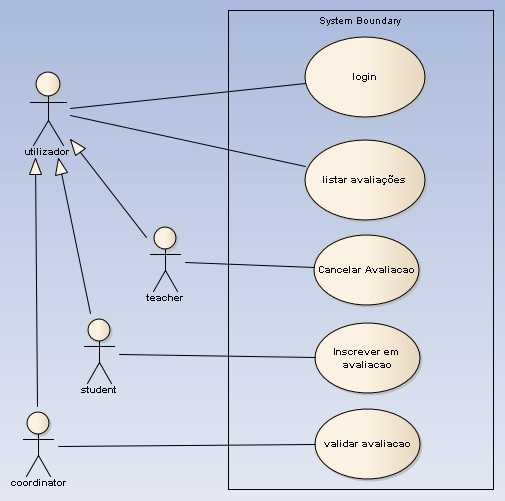
\includegraphics{imagens/casos_de_uso.jpg}
\caption{Diagrama: Casos de Uso}
\label{fig:casos_de_uso}
\end{figure}

\section{EFECTUAR LOGIN}
\subsection{Descrição}
Todos os utilizadores do sistema podem efectuar login ou logout do sistema. 

\subsection{Actores}
User

\subsection{Cenário Principal}
 
\subsubsection{Login}
\prettyref{fig:login}
O Utilizador:

1. Ao aceder ao site o sistema verifica se o utilizador está logado.

2. Caso o utilizador esteja logado:

2.1 O sistema consulta os cursos associados ao utilizador, agrupados pelo papel desempenhado no mesmo

2.2 O sistema consulta as disciplinas associadas ao utilizador para cada curso.

2.3 O sistema consulta as avaliações associadas a cada disciplina do utilizador

\subsection{Extensões ou Variações} 


\subsubsection{Logout}
 \prettyref{fig:logout}

O Utilizador:

1. Escolhe efectuar logout.

2. O sistema limpa os dados do utilizador na sessão actual.

3. O sistema limpa os cursos associados ao utilizador como coordinator.

4. O sistema limpa os cursos associados ao utilizador como teacher.

5. O sistema limpa os cursos associados ao utilizador como student.

\section{LISTAR AVALIAÇÕES}

\subsection{Descrição}
A cada acesso ao sistema, o mesmo consulta as avaliações associadas ao utilizador para semre apresentadas no calendário no intervalo de datas definido, bem como os detalhes das avaliações do dia seleccionado.

\subsection{Pré-condições}
O utilizador deverá estar logado e apenas terá acesso a avaliações a ele associadas como student, teacher ou coordinator.

\subsection{Actores}
User

\subsection{Cenário Principal}

\subsubsection{Listar avaliações entre datas} 
\prettyref{fig:listar_entre_datas}
O user:

1. Acede ao sistema, já logado.

2. O sistema obtem a lista de cursos a ele associados, passando pelos mesmo passos já descritos no login.

3. O sistema obtem o intervalo de datas definido.

4. O sistema obtem a lista de avaliações definidas no intervalo de datas.

5. É apresentado ao utilizador a lista de avaliações no calendário.

\subsection{Extensões ou Variações} 
\subsubsection{Listar detalhes de avaliações}
 \prettyref{fig:listar_detalhes}

O aluno:

1. Ao visualizar uma disciplina, escolhe cancelar a inscrição.

2. O sistema remove o registo na tabela AVALAÇÃO\_ALUNO.

3. O sistema obtem a lista de docentes da disciplina.

4. O sistema consulta o endereço de cada um dos docentes e envia um email com os detalhes da operação.

5. O sistema apresenta a mensagem de operação efectuada com sucesso ao aluno.

6. O sistema gera novamente a lista de avaliações para o intervalo de tempo actual.

7. É apresentado o painel de informações da avaliação e o calendário. 


\section{GERIR MOMENTO DE AVALIAÇÃO}
\subsection{Descrição} 
O docente pode criar, alterar e cancelar momentos de avaliação para as disciplinas em que seja docente.

\subsection{Pré-condições}
Apenas é possível criar momentos de avaliação para as disciplinas em que o docente esteja associado.

\subsection{Actores} 
Docente 

\subsection{Cenário Principal}
 \prettyref{fig:novo_momento_de_avaliacao} 
 \subsubsection{Novo Momento de Avaliação}
O Docente:

1. Escolhe criar um novo momento de avaliação.

2. É apresentado pelo sistema o formulário para inserir os dados

3. Em caso da operação correr com sucesso:

3.1 O sistema consulta os endereços de email do coordenador e dos restantes docentes da disciplina

3.2 É enviado uma mensagem para cada endereço a notificar a criação da avaliação

2.4 O sistema apresenta uma mensagem a informar do sucesso da operação

2.5 O sistema actualiza as informações do calendário

2.6 É apresentado novamente o calendário ao docente

4. Caso o aconteça um erro é apresentada a mensagem de erro ao docente.\\ 

\subsection{Extensões ou Variações} 
 \prettyref{fig:alterar_momento_de_avaliacao}
\subsubsection{Alterar Momento de Avaliação}

O Docente:

1. Escolhe Alterar um momento de Avaliação.

2. O sistema apresenta o formulário para as alterações.

3. O utilizador preenche o formulário.

4. O sistema regista as alterações à avaliação.

5. Caso a operação seja efectuada com sucesso:

5.1 O sistema consulta os endereços de email do coordenador do curso, restantes docentes e alunos da disciplina

5.2. O sistema envia uma mensagem para os endereços de email

5.3 O sistema apresenta uma mensagem a dar conta do sucesso da operação

6. Caso ocorra algum erro é apresentado o erro ao utilizador

\subsubsection{Cancelar Momento de Avaliação}
 \prettyref{fig:cancelar_momento_de_avaliacao}

O Docente:

1. Escolhe cancelar um momento de avaliação.

2. O sistema procede ao seu cancelamento.

3. Caso a operação ocorra com sucesso:

3.1. O sistema consulta os endereços de email do coordenador, dos restantes docentes e alunos da disciplina

3.2. O sistema envia uma mensagem para os endereços de email a dar conta do cancelamento

3.3 O sistema actualiza o calendário

3.4 O sistema apresenta uma mensagem a informar do sucesso da operação

3.5 O sistema apresenta o calendário actualizado

4. Caso ocorra algum erro, o mesmo é apresentado ao utilizador
\section{VALIDAR AVALIAÇÕES}

\subsection{Descrição}
O Coordenador de Curso pode validar, cancelar ou alterar as datas das avaliações das disciplinas do curso a ele associado 	

\subsection{Pré-condições}
O coordenador deverá estar logado e apenas terá acesso a avaliações de disciplinas do seu curso.

\subsection{Situações de Falha}
1. O Coordenador tenta validar uma avaliação já validada ou cancelar a validação de uma por validar.

\subsection{Actores}
Coordenador

\subsection{Cenário Principal}

\subsubsection{Validar Avaliação} 
\prettyref{fig:validar_avaliacao}
O coordenador:

1. Ao visualizar uma disciplina, escolhe validar.

2. O sistema regista a validação.

3. Caso a operação corra com sucesso:

3.1. O sistema obtem a lista de docentes e alunos da disciplina.

3.2. O sistema consulta o endereço de cada um dos docentes e envia um email com os detalhes da operação.

3.3. O sistema actualiza o calendario,

3.4. O sistema apresenta a mensagem de operação efectuada com sucesso ao coordenador.

3.5 O sistema apresenta o calendario

4. Caso ocorra algum erro, o mesmo é apresentado ao coordenador

\subsection{Extensões ou Variações} 
\subsubsection{Cancelar Validação}
 \prettyref{fig:cancelar_validacao}

O Coordenador:

1. Ao visualizar uma disciplina, escolhe cancelar a sua validação.

2. O sistema assinala a avaliação por validar

3. Caso a operação corra com sucesso:

3.1. O sistema obtem a lista de docentes e alunos da disciplina.

3.2. O sistema consulta o endereço de cada um dos docentes e envia um email com os detalhes da operação.

3.3. O sistema actualiza o calendário

3.4. O sistema apresenta a mensagem de operação efectuada com sucesso ao coordenador.

3.5 O sistema apresenta o calendário

4. Caso ocorra algum erro, o mesmo é apresentado ao coordenador.

\subsubsection{Alterar data de Momento de Avaliação}
 \prettyref{fig:alterar_data}

O Coordenador:

1. Ao visualizar uma avaliação, escolhe alterar a sua data.

2. O sistema apresenta o formulário para alterar a data da avaliação

3. O coordenador efectua a alteração

4. Caso a operação corra com sucesso:

4.1. O sistema obtem a lista de docentes e alunos da disciplina.

4.2. O sistema consulta o endereço de cada um dos docentes e envia um email com os detalhes da operação.

4.3. O sistema actualiza o calendário

4.4. O sistema apresenta a mensagem de operação efectuada com sucesso ao coordenador.

4.5 O sistema apresenta o calendário

5. Caso ocorra algum erro, o mesmo é apresentado ao coordenador.
\section{VISUALIZAR MOMENTO DE AVALIAÇÃO}

\subsection{Descrição}
Os utilizadores visualizam os momentos de avaliação associados ao seu perfil.	

\subsection{Pré-condições}
O utilizador deverá estar logado e apenas terá acesso a avaliações de disciplinas associadas ao seu perfil.

\subsection{Actores}
Utilizador

\subsection{Cenário Principal}

\subsubsection{Visualizar Momentos de Avaliação} 
\prettyref{fig:visualizar_momentos_de_avaliacao}
O Utilizador:

1. Ao aceder ao site é criado o calendário com base na data actual ou eventual data escolhida pelo mesmo.

2. O sistema consulta os momentos de avaliação associados ao perfil do utilizador.

3. O sistema apresenta o calendário ao utilizador

\subsection{Extensões ou Variações} 
\subsubsection{Visualizar Momento de Avaliação}
 \prettyref{fig:visualizar_momento_de_avaliacao}

O Utilizador:

1. Ao escolher um dia no calendário o sistema consulta as avaliações para esse dia 

2. O sistema apresenta o painel de opções de acordo com o seu perfil.

\subsubsection{Ver Detalhes de Momento de Avaliação}
 \prettyref{fig:visualizar_detalhes_de_momento_de_avaliacao}

O Utilizador:

1. No painel das avaliações do dia que escolheu anteriormente, clicka em ver detalhes da avaliação.

2. O sistema apresenta a janela com os detalhes da avaliação

\chapter{Modelação de Interfaces}

\section{Efectuar Login}
\begin{figure}[!htbp]
\centering
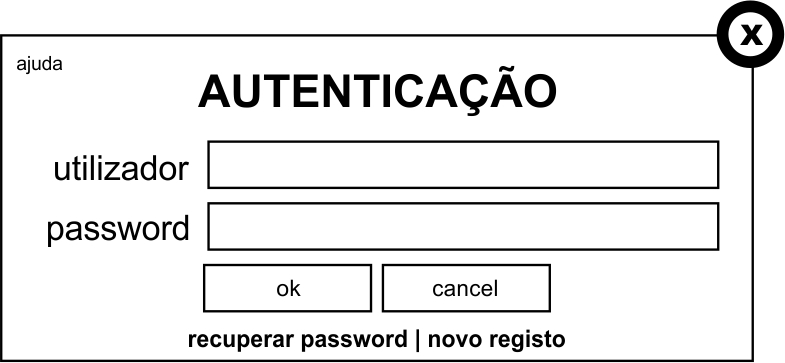
\includegraphics{imagens/login_i.jpg}
\caption{Storyboard: Login}
\label{fig:login_i}
\end{figure}

\begin{figure}[!htbp]
\centering
\includegraphics{imagens/logout_i.jpg}
\caption{Storyboard: Logout}
\label{fig:logout_i}
\end{figure}

\clearpage
\section{Gerir Inscrição em Momento de Avaliação}

\begin{figure}[!htbp]
\centering
\includegraphics{imagens/inscricao_avaliacao_i.jpg}
\caption{Storyboard: Efectuar Inscrição em Momento de Avaliação}
\label{fig:inscricao_avaliacao_i}
\end{figure}

\begin{figure}[!htbp]
\centering
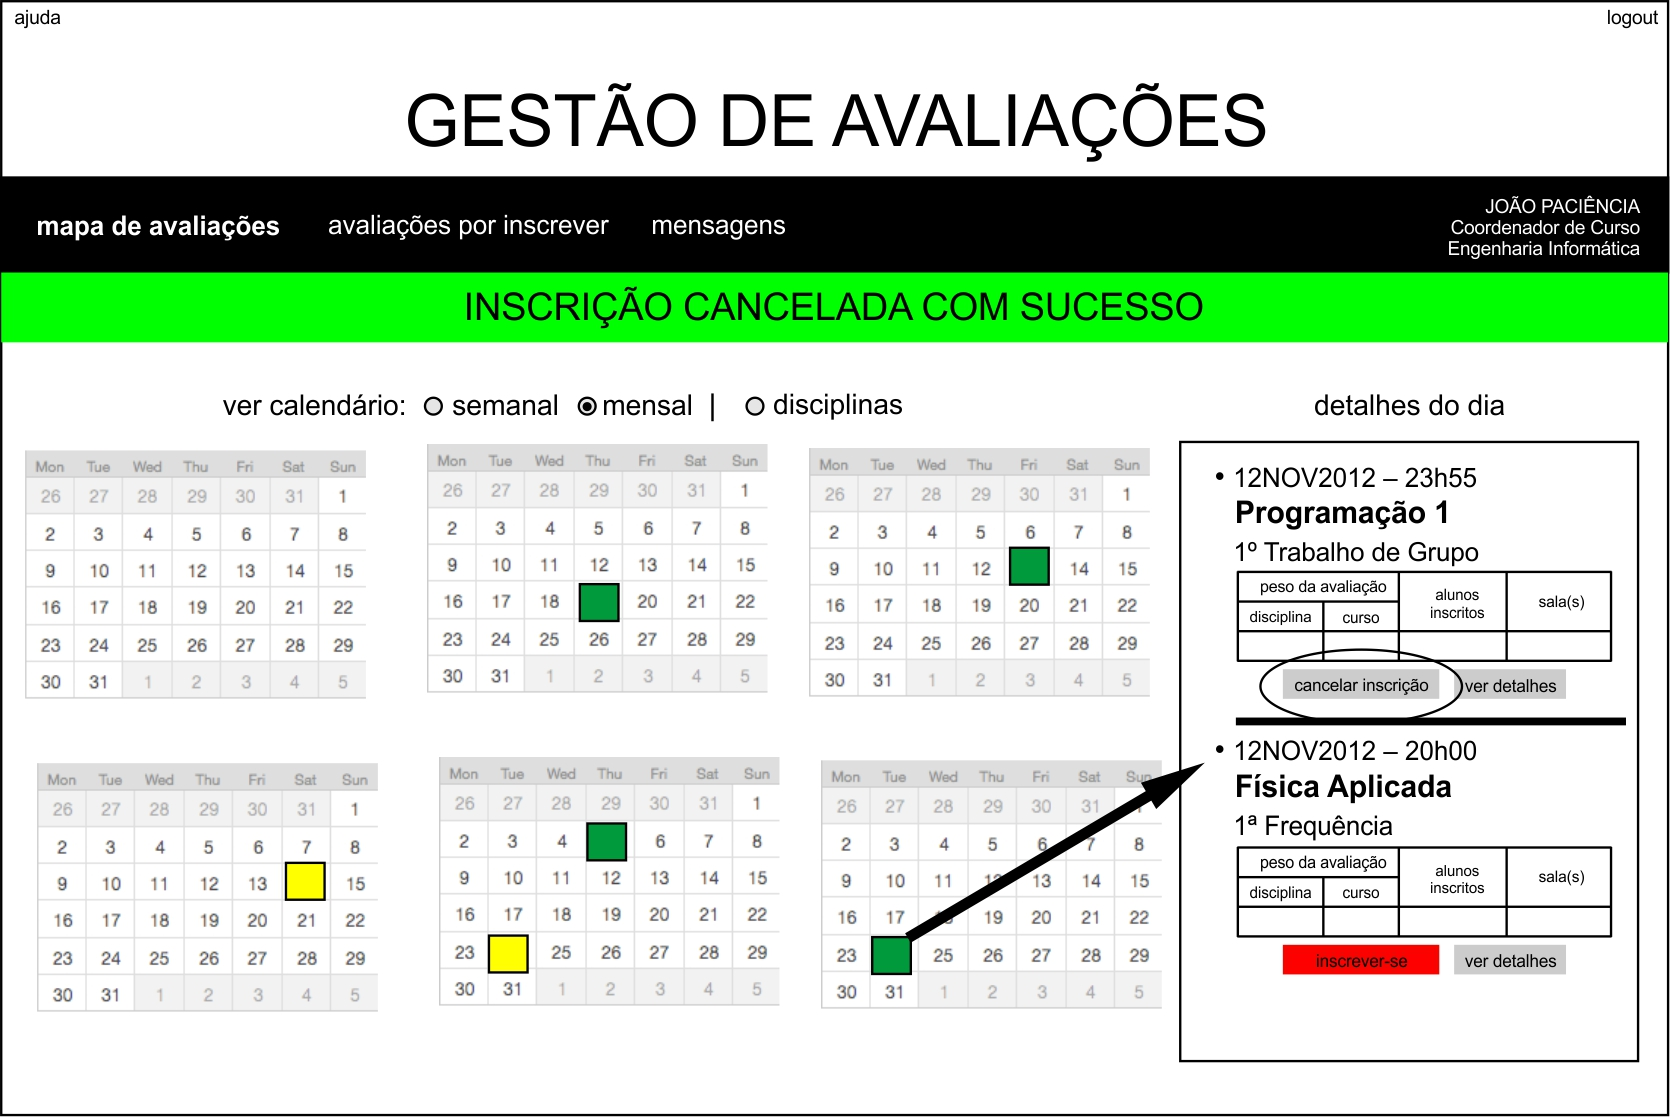
\includegraphics{imagens/cancelar_inscricao_i.jpg}
\caption{Storyboard: Cancelar Inscrição em Momento de Avaliação}
\label{fig:cancelar_inscricao_i}
\end{figure}



\clearpage
\section{Marcar Momento de Avaliação}

\begin{figure}[!htbp]
\centering
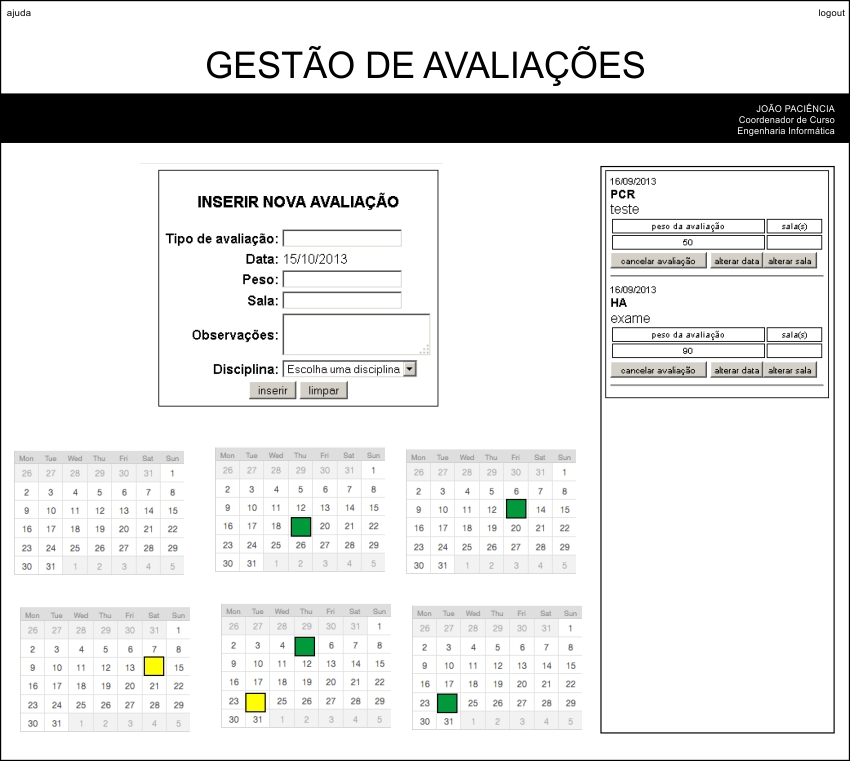
\includegraphics{imagens/nova_avaliacao_i.jpg}
\caption{Storyboard: Marcar Novo Momento de Avaliação}
\label{fig:nova_avaliacao_i}
\end{figure}

\begin{figure}[!htbp]
\centering
\includegraphics{imagens/cancelar_avaliacao_i.jpg}
\caption{Storyboard: Cancelar Momento de Avaliação}
\label{fig:cancelar_avaliacao_i}
\end{figure}

\clearpage
\section{Validar Momentos de Avaliação}

\begin{figure}[!htbp]
\centering
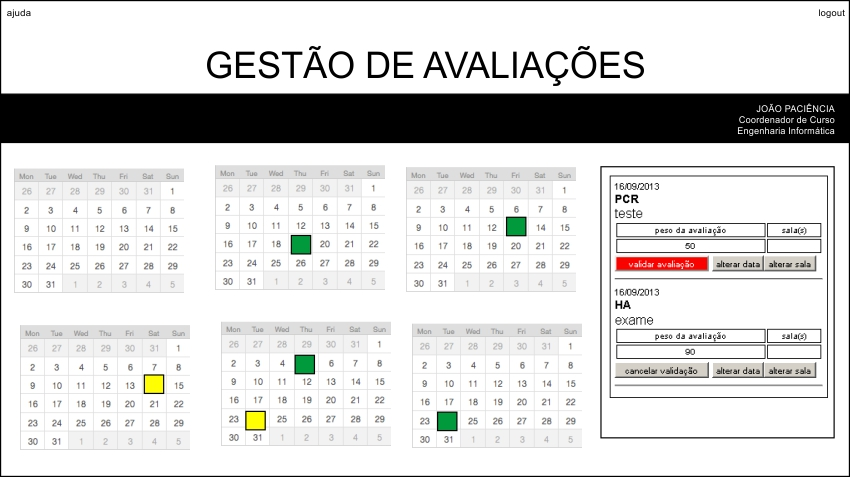
\includegraphics{imagens/validar_avaliacao_i.jpg}
\caption{Storyboard: Validar Momento de Avaliação}
\label{fig:validar_avaliacao_i}
\end{figure}

\begin{figure}[!htbp]
\centering
\includegraphics{imagens/cancelar_validacao_de_avaliacao_i.jpg}
\caption{Storyboard: Cancelar Validação de Momento de Avaliação}
\label{fig:cancelar_validacao_de_avaliacao_i}
\end{figure}

\clearpage
\section{Listar Momentos de Avaliação}

\chapter{Modelação da Base de Dados}

\paragraph{}

Resumidamente a base de dados está representada da seguinte forma:

\begin{list}{\textbf{-}}{\textbf{TABELAS}}
\item \textbf{curso} - Representa os cursos leccionados
\item \textbf{ano\_lectivo} - Representa um ano lectivo
\item \textbf{utilizador} - todos os utilizadores ficam registados nesta tabela
\item \textbf{curso\_ano} - Representa um curso leccionado num determinado ano, nesta tabela fica representado o coordenador do curso nesse ano associando o id do respectivo user na tabela utilizador
\item \textbf{semestre} - Representa um semestre de um determinado ano lectivo
\item \textbf{disciplina} - Representa uma disciplina
\item \textbf{disciplina\_semestre} - Faz referencia a uma disciplina leccionada num determinado semestre
\item \textbf{Docente} - Representa um ou mais utilizadores designados como docentes de uma determinada disciplina
\item \textbf{aluno} - Representa uma matrícula de um utilizador como aluno num determinado curso
\item \textbf{matricula\_disciplina} - Representa a matricula numa disciplina de um determinado aluno
\item \textbf{avaliacao} - Representa uma avaliacao marcada para uma disciplina leccionada num determinado semestre
\item \textbf{avaliacao\_datas\_alt} - Nesta tabela ficam registadas as datas alternati vas escolhidas pelo docente para que o coordenador possa ter a possibilidade de trocar caso aconteça um peso demasiado excessivo nas avaliações para os alunos.
\item \textbf{avaliacao\_aluno} - Representa a inscrição de um aluno numa avaliação e é onde fica registada a sua nota
\end{list}

\begin{list}{\textbf{-}}{\textbf{STORED PROCEDURES}}
\item \textbf{get_coordinator_evaluations} - Obter lista de avaliações com o perfil de coordenador de um determinado utilizador
\item \textbf{get_teacher_evaluations} - Obter lista de avaliações com o perfil de docente de um determinado utilizador
\item \textbf{get_student_evaluations} - Obter lista de avaliações com o perfil de aluno de um determinado utilizador
\item \textbf{get_cursos_user} - Obter lista de cursos a que utilizador esteja associado
\item \textbf{get_coordinator_disciplines} - Obter lista de disciplinas com o perfil de coordenador de um determinado utilizador
\item \textbf{get_teacher_disciplines} - Obter lista de disciplinas com o perfil de docente de um determinado utilizador
\item \textbf{get_student_disciplines} - Obter lista de disciplinas com o perfil de aluno de um determinado utilizador
\item \textbf{add_evaluation} - Adicionar uma avaliação a uma determinada disciplina
\end{list}

\begin{figure}[!htbp]
\centering
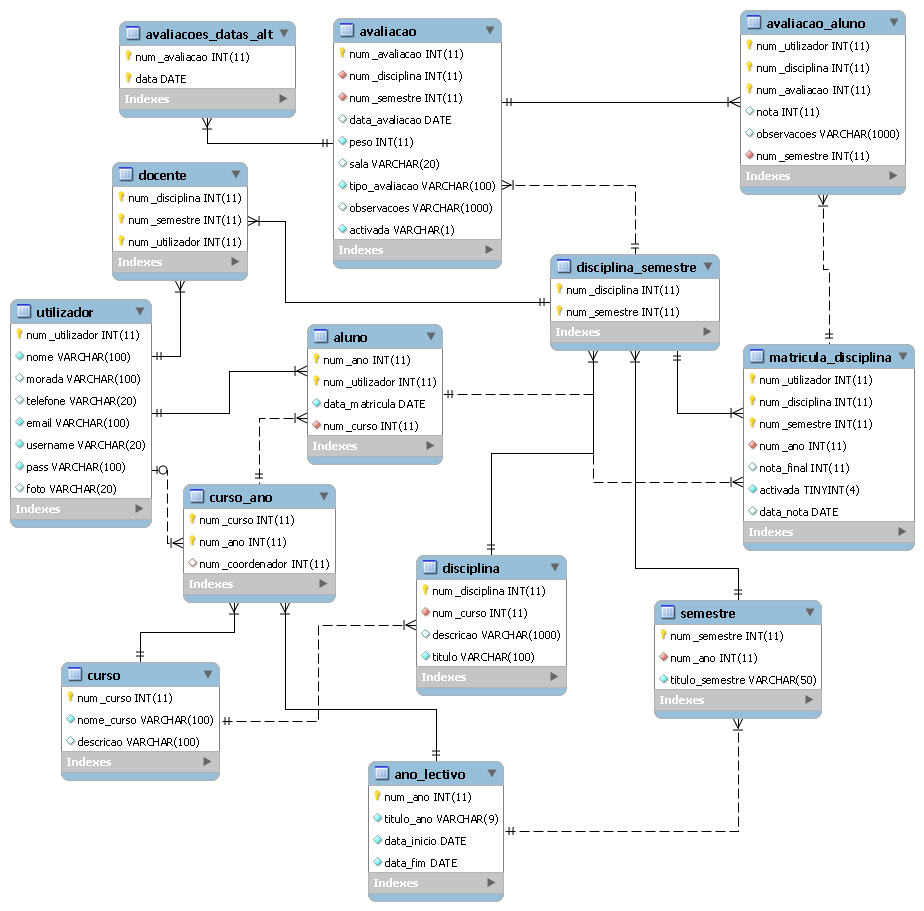
\includegraphics{imagens/base_de_dados.png}
\caption{Base de Dados: Modelo Físico}
\label{fig:modelo_fisico}
\end{figure}



\chapter{Modelação UML}

\section{Diagrama de Classes}
\begin{figure}[!htbp]
\centering
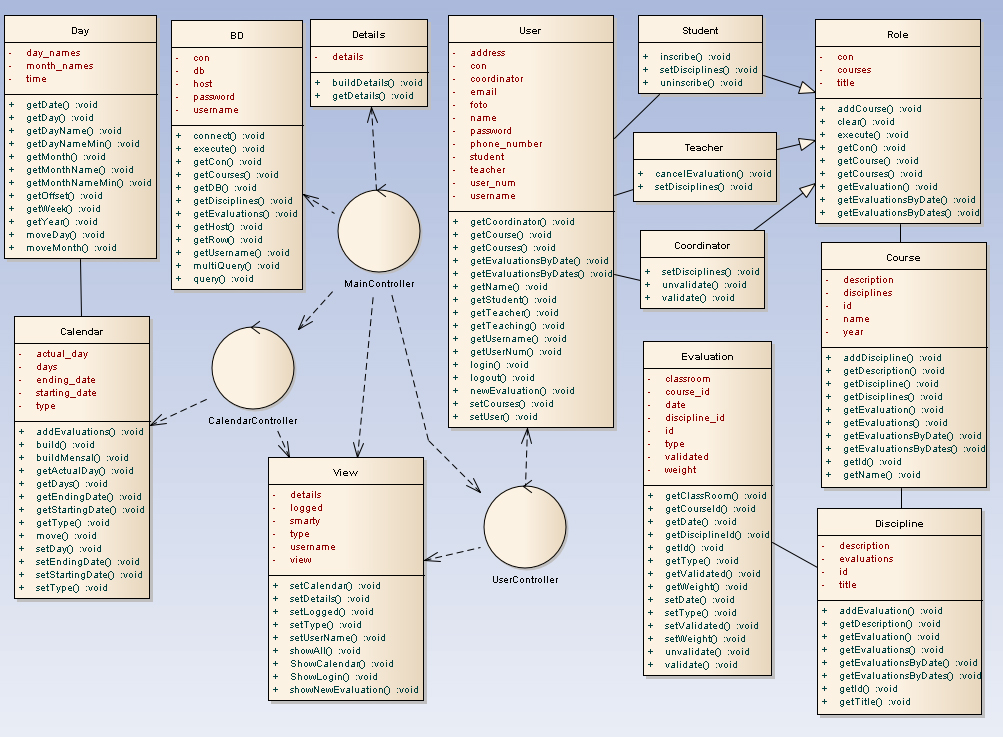
\includegraphics{imagens/diagrama_de_classes.jpg}
\caption{UML: Diagrama de Classes}
\label{fig:diagrama_de_classes}
\end{figure}

\section{Diagramas de Sequência}

\subsection{Efectuar Login}

\begin{figure}[!htbp]
\centering
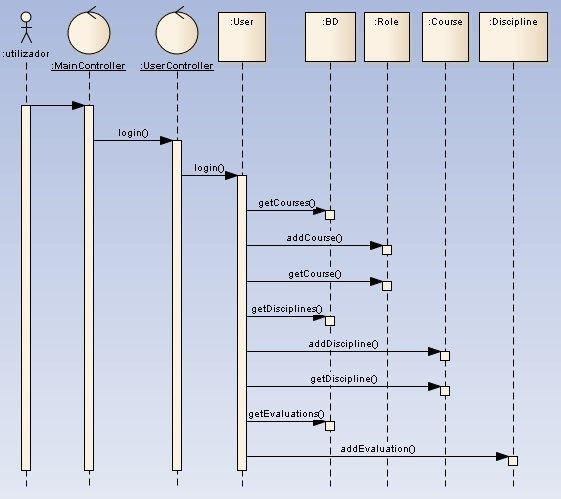
\includegraphics{imagens/login.jpg}
\caption{Diagrama de Sequência: Login}
\label{fig:login}
\end{figure}

\begin{figure}[!htbp]
\centering
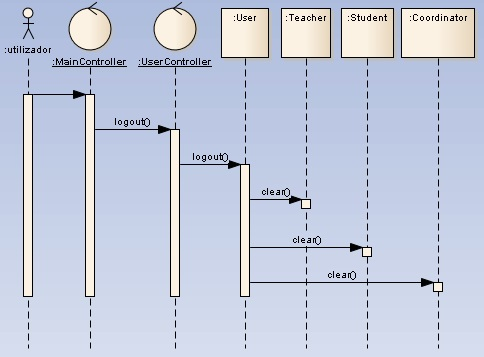
\includegraphics{imagens/logout.jpg}
\caption{Diagrama de Sequência: Logout}
\label{fig:logout}
\end{figure}

\clearpage
\subsection{Listar Avaliações}

\begin{figure}[!htbp]
\centering
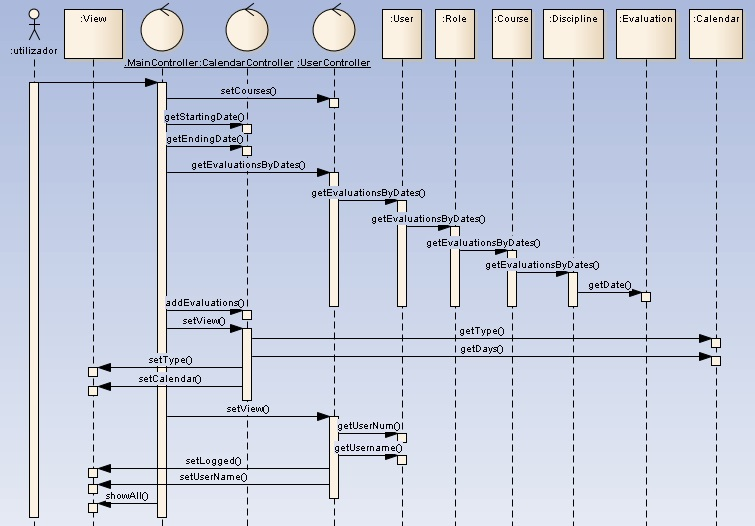
\includegraphics{imagens/listar_entre_datas.jpg}
\caption{Diagrama de Sequência: Listar Avaliações Entre Datas}
\label{fig:listar_entre_datas}
\end{figure}

\begin{figure}[!htbp]
\centering
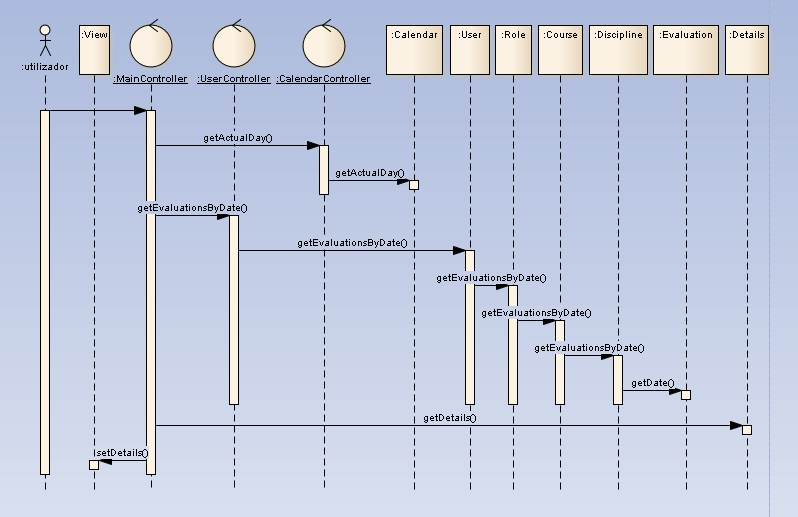
\includegraphics{imagens/listar_detalhes.jpg}
\caption{Diagrama de Sequência: Listar Detalhes de Avaliação}
\label{fig:listar_detalhes}
\end{figure}



\clearpage
\subsection{Inscrição em Avaliação}

\begin{figure}[!htbp]
\centering
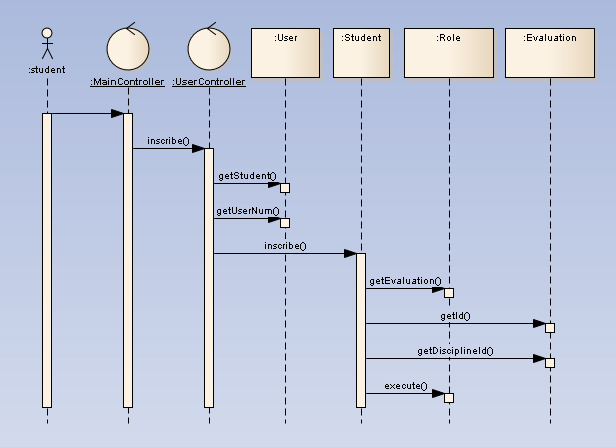
\includegraphics{imagens/inscrever_avaliacao.jpg}
\caption{Diagrama de Sequência: Efectuar Inscrição em Momento de Avaliação}
\label{fig:inscrever_avaliacao}
\end{figure}

\begin{figure}[!htbp]
\centering
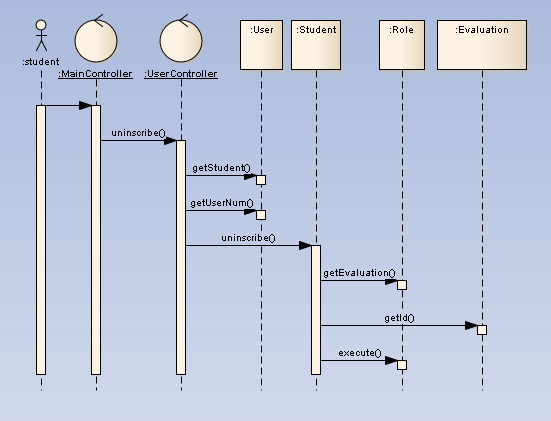
\includegraphics{imagens/cancelar_inscricao.jpg}
\caption{Diagrama de Sequência: Cancelar Inscrição de Momento de Avaliação}
\label{fig:cancelar_inscricao}
\end{figure}





\clearpage
\subsection{Marcar Avaliação}

\begin{figure}[!htbp]
\centering
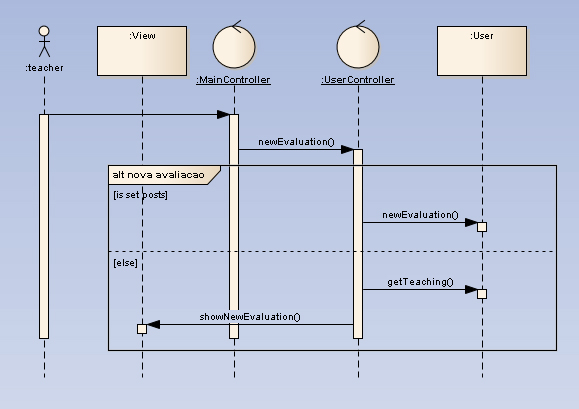
\includegraphics{imagens/nova_avaliacao.jpg}
\caption{Diagrama de Sequência: Novo Momento de Avaliação}
\label{fig:nova_avaliacao}
\end{figure}

\begin{figure}[!htbp]
\centering
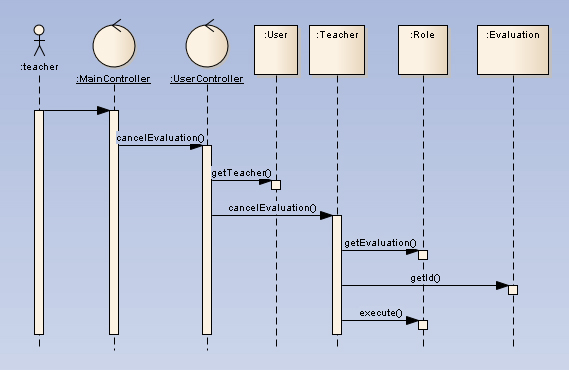
\includegraphics{imagens/cancelar_avaliacao.jpg}
\caption{Diagrama de Sequência: Cancelar Momento de Avaliação}
\label{fig:cancelar_avaliacao}
\end{figure}


\clearpage
\subsection{Validar Avaliações}

\begin{figure}[!htbp]
\centering
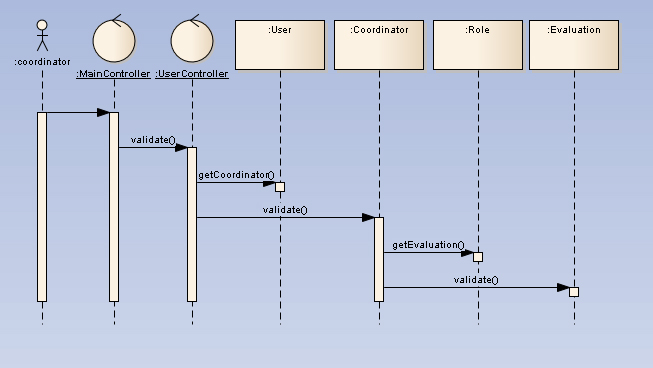
\includegraphics{imagens/validar_momento_de_avaliacao.jpg}
\caption{Diagrama de Sequência: Validar Avaliação}
\label{fig:validar_avaliacao}
\end{figure}

\begin{figure}[!htbp]
\centering
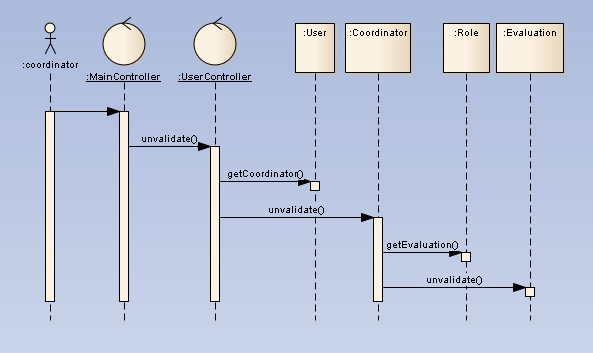
\includegraphics{imagens/cancelar_validacao.jpg}
\caption{Diagrama de Sequência: Cancelar Validação de Momento de Avaliação}
\label{fig:cancelar_validacao}
\end{figure}

%\chapter{Especificação de Requisitos}

\paragraph{}

\section{Requisitos Funcionais}

\subsection{Actores}

\subsubsection{Coordenador}

\subsubsection{Docente}

\subsubsection{Aluno}



\subsection{Casos de Uso}

\subsubsection{Gerir Inscrição em Momento de Avaliação}
	\textbf{Pré-Condições}\\
	O utilizador deve estar logado no sistema\\
	\textbf{Actores}\\
	Aluno\\
	\textbf{Cenário Principal}\\
	\textbf{Extensões ou Variações}\\

\subsubsection{Visualizar Momento de Avaliação}
	\textbf{Pré-Condições}\\
	O utilizador deve estar logado no sistema\\
	\textbf{Actores}\\
	Aluno, Coordenador e Docente\\
	\textbf{Cenário Principal}\\
	\textbf{Extensões ou Variações}\\

\subsubsection{Gerir Momento de Avaliação}
	\textbf{Pré-Condições}\\
	O utilizador deve estar logado no sistema\\
	\textbf{Actores}\\
	Docente\\
	\textbf{Cenário Principal}\\
	\textbf{Extensões ou Variações}\\



\subsubsection{Validar Avaliações}
	\textbf{Pré-Condições}\\
	O utilizador deve estar logado no sistema\\
	\textbf{Actores}\\
	Coordenador\\
	\textbf{Cenário Principal}\\
	\textbf{Extensões ou Variações}\\

\subsection{Diagrama de Classes}
(Seitz, 2009) \cite{seitz09:_gray_hat_python}.

\subsection{Base de Dados}
O modelo físico da Base de Dados pode ser consultado na \prettyref{fig:modelofisico}
\begin{figure}[h]
\centering
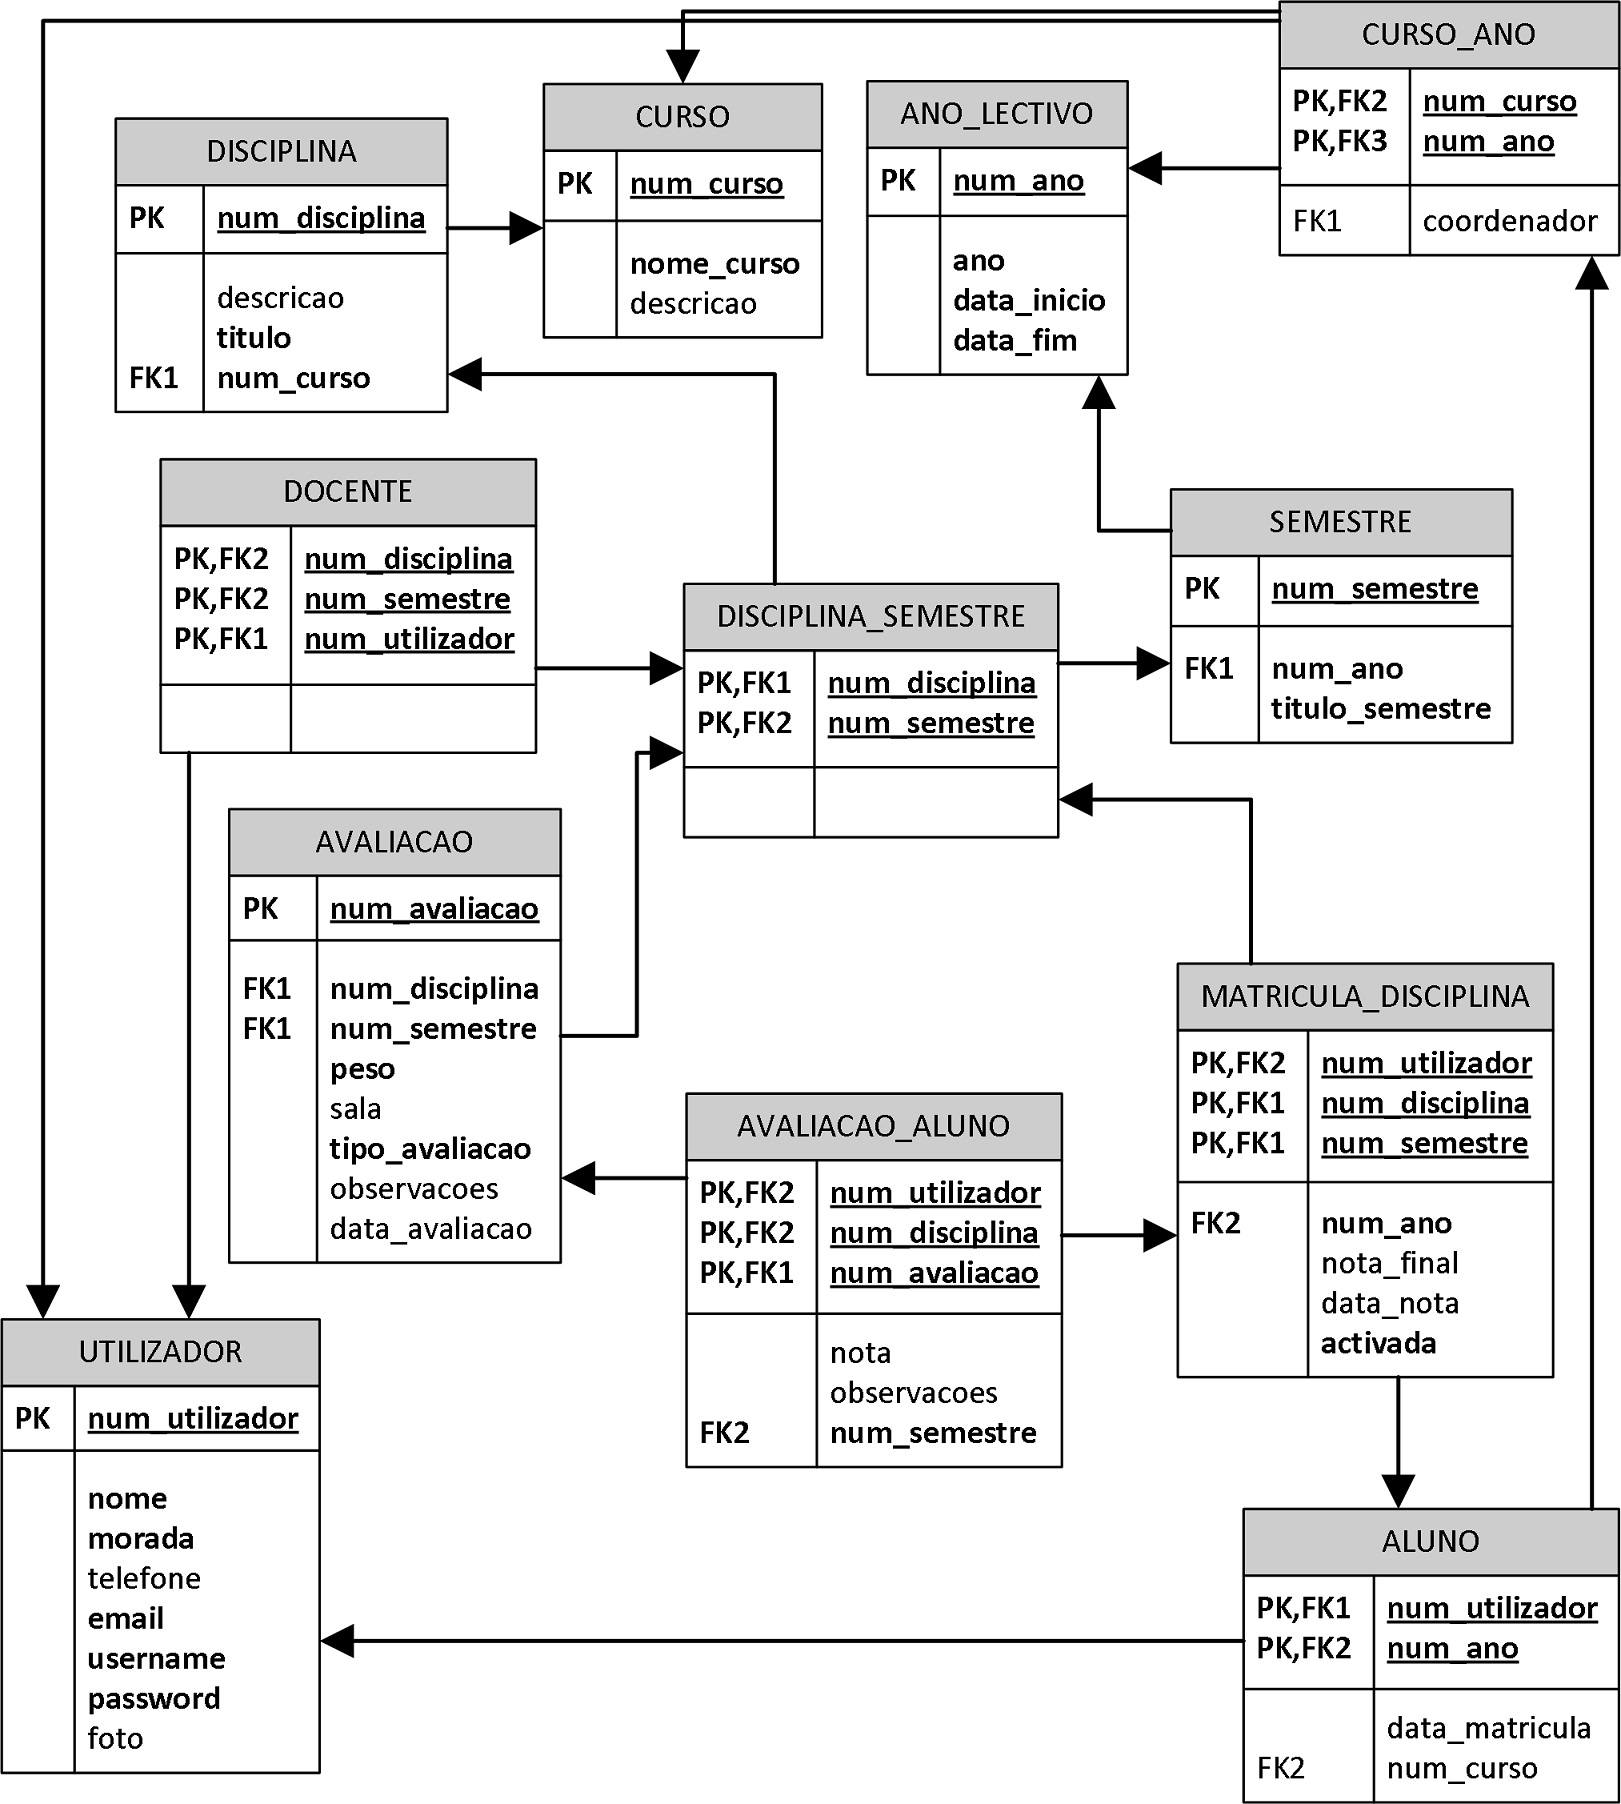
\includegraphics{imagens/modelofisico.jpg}
\caption{Base de Dados: Modelo Físico}
\label{fig:modelofisico}
\end{figure}
\section{Requisitos Não Funcionais}

\subsection{Requisitos do Produto}
O site a construir deverá respeitar os principais princípios e regras de Usabilidade e Acessibilidade, sendo que no último caso deverá respeitar o nível AA.
A autenticação dos membros deve ser efectuada através de sessões seguras.

\subsection{Requisitos Organizacionais}
O site será implementado em duas linguagens, PHP e ASP.NET utilizando bases de dados mySQL. Na versão PHP irão ser utilizados os API\'s jQuery e Smarty 



%\input{analise}
% As 11 questões da análise de Tarefas
% Análise Hierárquica
%   Coordenador / Docente / Aluno
% Cenários do Problema
%   Coordenador / Docente / Aluno

%\input{desenho}
% Cenários de Interacção
%  Cordenador / Docente / Aluno
% Definição de métricas de usabilidade
% Protótipo não funcional
%   Storyboards
%   Wireframes

%\chapter{Apêndices}
\section{index.php}
\lstinputlisting[language=PHP]{ficheiros/index.php}

\section{controller/MainController.php}
\lstinputlisting[language=PHP]{ficheiros/controller/MainController.php}
\section{controller/UserController.php}
\lstinputlisting[language=PHP]{ficheiros/controller/UserController.php}
\section{controller/CalendarController.php}
\lstinputlisting[language=PHP]{ficheiros/controller/CalendarController.php}


\section{model/BD.php}
\lstinputlisting[language=PHP]{ficheiros/model/BD.php}
\section{model/Calendar.php}
\lstinputlisting[language=PHP]{ficheiros/model/Calendar.php}
\section{model/Coordinator.php}
\lstinputlisting[language=PHP]{ficheiros/model/Coordinator.php}
\section{model/Course.php}
\lstinputlisting[language=PHP]{ficheiros/model/Course.php}
\section{model/Day.php}
\lstinputlisting[language=PHP]{ficheiros/model/Day.php}
\section{model/Details.php}
\lstinputlisting[language=PHP]{ficheiros/model/Details.php}
\section{model/Evaluation.php}
\lstinputlisting[language=PHP]{ficheiros/model/Evaluation.php}
\section{model/Role.php}
\lstinputlisting[language=PHP]{ficheiros/model/Role.php}
\section{model/Student.php}
\lstinputlisting[language=PHP]{ficheiros/model/Student.php}
\section{model/Teacher.php}
\lstinputlisting[language=PHP]{ficheiros/model/Teacher.php}
\section{model/User.php}
\lstinputlisting[language=PHP]{ficheiros/model/User.php}

\section{view/View.php}
\lstinputlisting[language=PHP]{ficheiros/view/View.php}

\section{css/simple.css}
\lstinputlisting[language=HTML]{ficheiros/css/simple.css}

\section{scripts/codes.js}
\lstinputlisting[language=HTML]{ficheiros/scripts/codes.js}

\section{templates/b\_login.tpl}
\lstinputlisting[language=HTML]{ficheiros/templates/b_login.tpl}
\section{templates/coordinator\_details.tpl}
\lstinputlisting[language=HTML]{ficheiros/templates/coordinator_details.tpl}
\section{templates/detalhes\_avaliacao.tpl}
\lstinputlisting[language=HTML]{ficheiros/templates/detalhes_avaliacao.tpl}
\section{templates/detalhes.tpl}
\lstinputlisting[language=HTML]{ficheiros/templates/detalhes.tpl}
\section{templates/identificacao.tpl}
\lstinputlisting[language=HTML]{ficheiros/templates/identificacao.tpl}
\section{templates/index.tpl}
\lstinputlisting[language=HTML]{ficheiros/templates/index.tpl}
\section{templates/menu.tpl}
\lstinputlisting[language=HTML]{ficheiros/templates/menu.tpl}
\section{templates/monthly.tpl}
\lstinputlisting[language=HTML]{ficheiros/templates/monthly.tpl}
\section{templates/new\_evaluation.tpl}
\lstinputlisting[language=HTML]{ficheiros/templates/new_evaluation.tpl}
\section{templates/painel\_login.tpl}
\lstinputlisting[language=HTML]{ficheiros/templates/painel_login.tpl}
\section{templates/rodape.tpl}
\lstinputlisting[language=HTML]{ficheiros/templates/rodape.tpl}
\section{templates/student\_details.tpl}
\lstinputlisting[language=HTML]{ficheiros/templates/student_details.tpl}
\section{templates/teacher\_details.tpl}
\lstinputlisting[language=HTML]{ficheiros/templates/teacher_details.tpl}
\section{templates/teacher\_menu.tpl}
\lstinputlisting[language=HTML]{ficheiros/templates/teacher_menu.tpl}




\chapter{Conclusão}

\paragraph{}

O trabalho apresentado neste relatório, resultou num site onde é possivel gerir momentos de avaliação de cursos leccionados no IPBeja. É possivel um utilizador seguir com o mesmo registo ao longo do tempo, podendo assumir os papéis de Aluno, Docente e/ou Coordenador de Curso.\\
É possivel ao utilizador visualizar as avaliações relacionadas com os papéis por ele desempenhados e, mais especificamente, enquanto Coordenador de Curso: validar ou cancelar a validação de uma avaliação, enquanto Docente: marcar ou cancelar a marcação de uma avaliação e enquanto Aluno: inscrever-se ou cancelar a inscrição num momento de avaliação.\\
Para gerar as página html foi utilizado o motor de templates \code{smarty} que torna mais simples e de melhor compreensão essas tarefas.\\
Por uma questão de segurança, com o intuito de evitar erros de programação ou acessos indevidos, foram criados stored procedures para controlar o acesso ou alterações aos momentos de avaliação.\\
Como trabalho futuro deverá ser implementada uma forma de criação de um login à base de dados para cada utilizador para que se possa limitar o acesso directo às tabelas e o mesmo seja apenas feito através de stored procedures onde será utilizado como referência para as permissões de acesso aos dados o utilizador logado ao invés da disponibilização do id de utilizador como está feito actualmente.

\end{document} 